
\documentclass[11pt,a4paper,sans]{moderncv}        % possible options include font size ('10pt', '11pt' and '12pt'), paper size ('a4paper', 'letterpaper', 'a5paper', 'legalpaper', 'executivepaper' and 'landscape') and font family ('sans' and 'roman')

% moderncv themes
\moderncvstyle{banking}                             % style options are 'casual' (default), 'classic', 'banking', 'oldstyle' and 'fancy'
\moderncvcolor{black}                               % color options 'black', 'blue' (default), 'burgundy', 'green', 'grey', 'orange', 'purple' and 'red'
%\renewcommand{\familydefault}{\sfdefault}         % to set the default font; use '\sfdefault' for the default sans serif font, '\rmdefault' for the default roman one, or any tex font name
%\nopagenumbers{}                                  % uncomment to suppress automatic page numbering for CVs longer than one page

% character encoding
\usepackage[utf8]{inputenc}                       % if you are not using xelatex ou lualatex, replace by the encoding you are using
%\usepackage{CJKutf8}                              % if you need to use CJK to typeset your resume in Chinese, Japanese or Korean

% adjust the page margins
\usepackage[scale=0.75, top=2cm]{geometry}
% \setlength{\hintscolumnwidth}{3cm}                % if you want to change the width of the column with the dates
%\setlength{\makecvtitlenamewidth}{10cm}           % for the 'classic' style, if you want to force the width allocated to your name and avoid line breaks. be careful though, the length is normally calculated to avoid any overlap with your personal info; use this at your own typographical risks...

\usepackage{pdfpages}

% personal data
\name{Luke}{Kokoftopoulos}
% \title{Resumé title}                               % optional, remove / comment the line if not wanted
\address{Software Engineer}{University of Technology Sydney}% optional, remove / comment the line if not wanted; the "postcode city" and "country" arguments can be omitted or provided empty
\phone[mobile]{0478 790 532}                   % optional, remove / comment the line if not wanted; the optional "type" of the phone can be "mobile" (default), "fixed" or "fax"
% \phone[fixed]{+2~(345)~678~901}
% \phone[fax]{+3~(456)~789~012}
\email{luke.d.kokoftopoulos@student.uts.edu.au}                               % optional, remove / comment the line if not wanted
% \homepage{www.johndoe.com}                         % optional, remove / comment the line if not wanted
\social[linkedin]{lukekoko}                        % optional, remove / comment the line if not wanted
% \social[twitter]{jdoe}                             % optional, remove / comment the line if not wanted
\social[github]{lukekoko}                              % optional, remove / comment the line if not wanted
% \extrainfo{additional information}                 % optional, remove / comment the line if not wanted
% \photo[64pt][0.4pt]{picture}                       % optional, remove / comment the line if not wanted; '64pt' is the height the picture must be resized to, 0.4pt is the thickness of the frame around it (put it to 0pt for no frame) and 'picture' is the name of the picture file
% \quote{Some quote}                                 % optional, remove / comment the line if not wanted

% bibliography adjustements (only useful if you make citations in your resume, or print a list of publications using BibTeX)
%   to show numerical labels in the bibliography (default is to show no labels)
\makeatletter\renewcommand*{\bibliographyitemlabel}{\@biblabel{\arabic{enumiv}}}\makeatother
%   to redefine the bibliography heading string ("Publications")
%\renewcommand{\refname}{Articles}

% bibliography with mutiple entries
%\usepackage{multibib}
%\newcites{book,misc}{{Books},{Others}}
%----------------------------------------------------------------------------------
%            content
%----------------------------------------------------------------------------------
\begin{document}
%-----       resume       ---------------------------------------------------------
\makecvtitle
\vspace*{-10mm}

\section{Education}
\cventry{January 2017--November 2021}{Bachelor of Engineering(Honours) in Software}{University of Technology Sydney}{}{}{Sub-major in Data Analytics with a focus in Machine Learning}
\cventry{January 2017--November 2021}{Diploma in Professional Engineering Practice}{University of Technology Sydney}{}{}{}  

\section{Engineering Capstone}
\cvitem{Title}{\emph{Software Security Analysis using Deep Learning}}
\cvitem{Supervisors}{Yulei Sui}
\cvitem{Description}{The project aim is to develop new techniques to detect and repair software security vulnerabilities for large and real-world software projects by leveraging deep learning and natural language processing.}

\section{Experience}
\cventry{February 2020--Current}{Junior Support Engineer}{GTSGroup}{}{}{
\begin{itemize}
\item OSIsoft PI System support for various clients; fixing system issues and performing system health checks.
\item Created various ETL Python scripts for clients.
\item Designed and developed a program in Python to fetch data from PI System, then publish data to Google Sheets.
\item Working in a project team to setup, install and customise PI System for clients.
\end{itemize}}

\cventry{January 2019--January 2020}{Engineer Undergraduate - Software}{Veolia Australia and New Zealand}{}{}{
\begin{itemize}
\item Developed web scrapers in Python to get weather data and data from meters such as power meters and flow meters into PI System.
\item Pre-processing various data forms; csv, excel and json. With Python for ingest into PI System.
\item Implemented an email attachment downloader in Python to download files from emails. Saving time for the company as this was done manually by an engineer on a daily basis.  
\item Systems support for OSIsoft PI System; fixing system issues and enhancing functionality 
\end{itemize}}

\cventry{August 2018-- January 2019}{Software Engineering Intern}{Veolia Australia and New Zealand}{}{}{
\begin{itemize}
\item Designed and Developed web application for internal users to input data into PI System using Angular, Node.js and Microsoft SQL Server.
\item Systems support for OSIsoft PI System; fixing system issues and enhancing functionality 
\end{itemize}}

\cventry{February 2017-- August 2018}{Service Team Member}{Coles Roselands}{}{}{
\begin{itemize}
\item Serving customers, handling money, packing shopping bags and arringing stock on shelves.
\end{itemize}}


\section{Technical Skills}
\cvitemwithcomment{Programming}{Python, JavaScript, TypeScript, C, C++, C\#, Java, MSSQL, MySQL,}{}
\cvitemwithcomment{}{HTML, CSS}{}
\cvitemwithcomment{Frameworks}{Angular, React, Node.js, Express.js, Flask, Django, Docker, GCP, Firebase, AWS}{}
\cvitemwithcomment{Data Science}{TensorFlow, Keras, Pandas, Scikit-Learn, NumPy}{}
\cvitemwithcomment{Tools}{Git, GitHub, Travis CI, Excel, Jira, Trello}{}
\cvitemwithcomment{Systems}{OSIsoft PI System(Real-time data management system); PI AF, PI Vison,}{}
\cvitemwithcomment{}{PI Web API, PI UFL Interface, PI Datalink}{}

\section{Transferable Skills}
\cvlistitem{Strong \textbf{problem solving} skill demonstrated by being a system support engineer. I regularly solve various customer problems relating to systems issues. I have also developed many ETL scripts that solve problems with data ingest to the PI System.}
\cvlistitem{Ability to work in a \textbf{team} and \textbf{independently} shown through employment at GTSGroup and Veolia. I have also worked in a variety of teams in the 6 Software Engineering Studios I have completed at university where I got a high distinction mark. }
\cvlistitem{Strong \textbf{communication} and \textbf{listening} skills demonstrated through employment at GTSGroup, Veolia and Coles. I communicate through email, phone, online meetings and in person to colleagues and clients.}
\cvlistitem{\textbf{Fast learner} shown by the ability to learn new tools and software quickly. I am constantly learning new software libraries and frameworks at work and university.}
\cvlistitem{Efficient \textbf{time management} shown by completing system support tickets within the resolution time at GTSGroup.}
\cvlistitem{Ability to \textbf{work under pressure} shown by working in a fast paced service environment at Coles.}


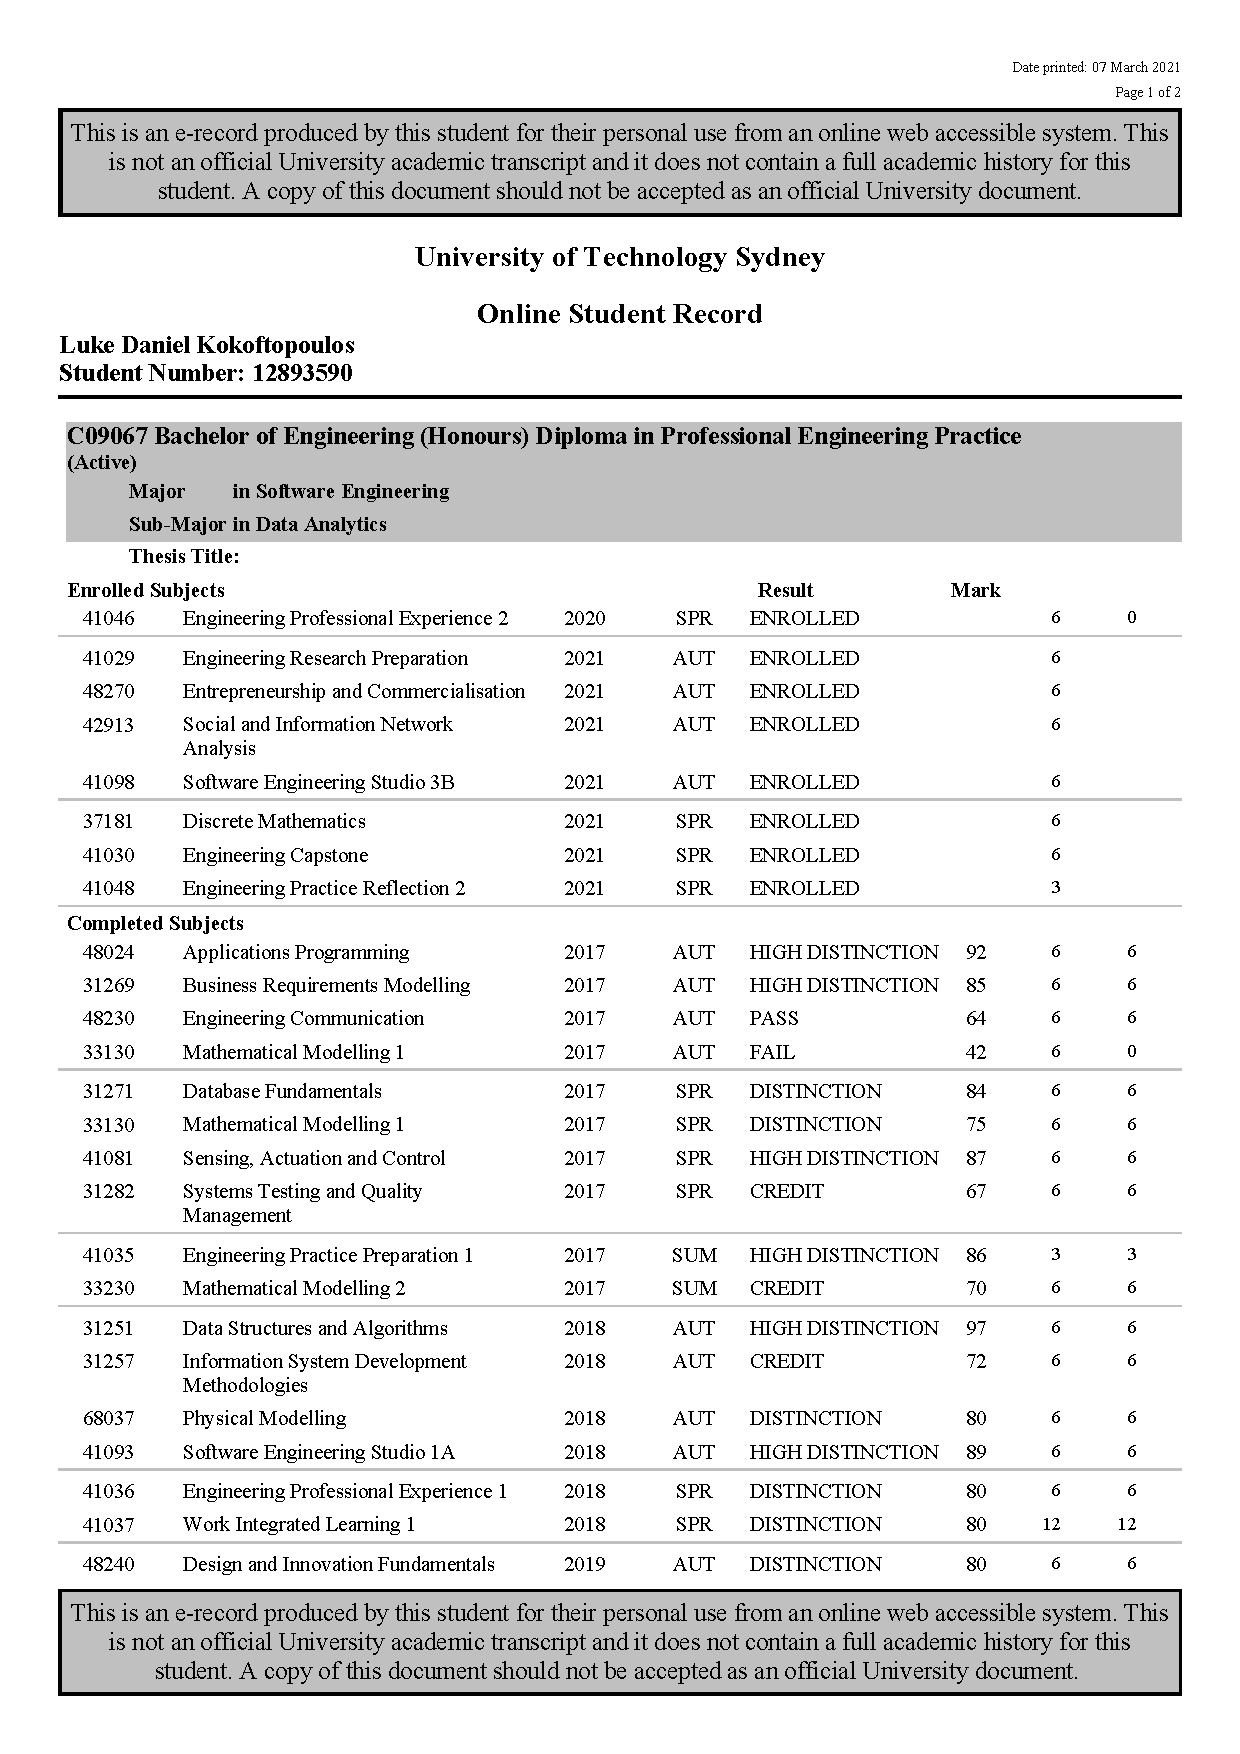
\includepdf[pages=-]{transcript.pdf}

\clearpage
\end{document}
